% SOICT 2026 submission — Springer CCIS format (single-blind: keep author names).
% Requires the Springer LNCS/CCIS class `llncs.cls` + `splncs04.bst` from
% https://soict.org/wp-content/uploads/2025/09/Latex-Template-for-Springer.zip
% Max 12 pages excluding references. Figure: convert docs/paper/diagrams/soict_harlstmgat.svg -> PDF.
% Cross-market version: VN30/VN100 main + HOSE/HNX OOS + S&P 500 cross-market check.
\documentclass[runningheads]{llncs}
\usepackage{graphicx}
\graphicspath{{diagrams/}}   % figure lives in docs/paper/diagrams/ (do NOT add ./ — collides with output pdf)
\usepackage{booktabs}
\usepackage{amsmath}
\usepackage[T1]{fontenc}

\begin{document}

\title{Multi-Horizon Stock Volatility Forecasting}

\author{Author One\inst{1} \and Author Two\inst{1}}
\authorrunning{Multi-Horizon Volatility Forecasting}
\institute{Affiliation, City, Country \\ \email{\{author1,author2\}@example.edu}}

\maketitle

\begin{abstract}
Forecasting how much a stock's price will swing from one day to the next --- its \emph{volatility} --- is a
basic input to risk management, option pricing, and portfolio decisions. The standard benchmark, the HAR model,
is a simple regression that predicts tomorrow's volatility from its own recent daily, weekly, and monthly
averages, treating each stock in isolation. Deep sequence models and graph neural networks are widely expected
to improve on it --- the former by capturing non-linear patterns in a stock's own history, the latter by letting
related stocks share information so that turbulence in one can inform another --- yet whether either forecasts
better out of sample, and at which horizons, remains unsettled, with many reported gains resting on evaluation
choices that flatter the more complex model.
We test this directly, using the Vietnamese equity market as a case study. Giving every model the same five
inputs, we compare the linear HAR benchmark against a deep sequence model (an LSTM) and against that same model
extended with a graph-attention branch that links each stock to a few related peers. All models forecast a
high--low range measure of daily volatility (the Parkinson estimator, a variance) at one, five, ten, and
twenty-two trading days ahead, judged by five standard error measures and a significance test adapted to the
fact that stocks move together. On the liquid VN30 and VN100 indices the simple HAR benchmark is the most
accurate on the volatility-specific error at every horizon, with no learned model significantly better, although
the deep models lead on absolute error at the shortest horizon. Re-running the identical, un-retuned setup on the
broader Vietnamese market and on the U.S. S\&P 500 shows the outcome depends on liquidity: on the thinly traded
HNX exchange the deep and graph models become significantly more accurate than HAR at several horizons, while on
liquid markets HAR remains hard to beat, and adding the graph rarely improves on the deep model beyond
training-seed noise. We report every result with explicit data-quality caveats rather than as a uniform win.
\keywords{Volatility forecasting \and HAR \and LSTM \and Graph Attention Network \and Diebold--Mariano.}
\end{abstract}

\section{Introduction}
Financial markets are volatile: prices swing, and the size of those swings --- an asset's \emph{volatility} ---
is the standard measure of its risk. Because volatility drives how options are priced, how much capital a
position ties up, and how risk is budgeted across a portfolio, forecasting it accurately is a long-standing
problem in financial econometrics~\cite{corsi2009}. Volatility is not observed directly; it is estimated from
prices, so any forecast is a forecast of an estimate. We target the daily \emph{Parkinson estimator}, which
gauges a day's variance from its high--low price range and uses more of the day's information than a
close-to-close measure; our forecasting target is therefore a variance (a squared quantity), not a standard
deviation.

The dominant benchmark is the HAR model~\cite{corsi2009}: a plain linear regression that predicts tomorrow's
volatility from its own averages over the last day, the last week (about five trading days), and the last month
(about twenty-two), summarising volatility's long memory with a handful of coefficients. HAR is deliberately
simple and famously hard to beat, but it has a structural blind spot --- it treats each stock on its own and
ignores that stocks in the same market move together, so a shock in one stock is never allowed to inform a
forecast for another.

Two model families are widely proposed to close that gap. Sequence models such as the LSTM~\cite{lstm1997}
learn non-linear patterns in a stock's own history, and graph neural networks --- here a Graph Attention Network
(GAT)~\cite{gat2018} --- model \emph{cross-sectional spillover}, the same-day spread of turbulence from one stock
to related ones, by letting each stock draw on an attention-weighted average of its most relevant peers. Whether
these additions actually improve out-of-sample volatility forecasts is, however, mixed in the literature, and
reported gains are often confounded by evaluation choices --- for example restricting the sample to the dates on
which every stock is simultaneously present (which discards most of the data), or counting many co-moving stocks
as independent evidence (which overstates statistical significance).

This paper measures, under one leakage-free evaluation, whether temporal non-linearity or a cross-sectional
graph changes the forecast relative to a linear benchmark. Holding the five inputs and the data design fixed, we
compare an extended HAR (HAR-X), an LSTM, and an LSTM+GAT on the Vietnamese VN30 and VN100 indices, with
GARCH(1,1) as a classical reference, and repeat the identical protocol --- without any retuning --- on the wider
Vietnamese market (the HOSE and HNX exchanges) and on the U.S. S\&P 500. To keep the comparison fair we evaluate
on a \emph{masked panel}: instead of intersecting to the dates on which every stock is present, we keep the union
of trading dates and mask stocks not yet listed on a given date, so every model sees the same panel and the same
five features. Our headline finding is candid rather than a uniform win: on liquid markets the simple HAR-X is
the most accurate on the volatility-specific error at every horizon, while the value of the deep and graph
components concentrates in the less-liquid HNX market.

Our contributions are: (i) a multi-horizon, multi-seed benchmark that holds the feature set and data design fixed
across HAR-X, an LSTM, and an LSTM+GAT, so any measured difference is attributable to a single component; (ii) a
component-by-component reading of when the temporal and graph parts help --- HAR-X has the lowest
volatility-specific error on the liquid panels with no learned model significantly better, whereas on the
less-liquid HNX exchange the deep and graph models are significantly more accurate at several horizons, and the
graph rarely improves on the plain LSTM beyond training-seed noise; and (iii) a panel-correct significance
protocol --- because co-moving stocks are not independent, we cluster the Diebold--Mariano test by date, since a
naive per-stock test overstates significance roughly in proportion to the square root of the number of stocks.
Every reported number is taken from a stored results file, and we document the data-quality limitations ---
notably the high share of zero-range (no-intraday-move) days on the illiquid exchange and the unverified split
adjustment of the Vietnamese prices --- rather than presenting the data as uniformly clean.

\paragraph{Terminology (for readers outside finance).}
\emph{Volatility}: the size of a stock's price fluctuations, the standard proxy for its risk.
\emph{Parkinson estimator}: a day's variance measured from its high--low price range; our forecasting target is
this variance (squared units), not the standard deviation.
\emph{HAR}: a linear model predicting volatility from its own daily, weekly, and monthly averages.
\emph{GARCH}: a classical time-series model that carries variance forward from recent return shocks.
\emph{QLIKE}: an error measure designed for volatility that stays reliable when the target is a noisy proxy and
penalises under-forecasting of risk more heavily than over-forecasting.
\emph{Diebold--Mariano (DM) test}: a test of whether one forecast is more accurate than another by more than
chance, computed from their day-by-day loss differences.
\emph{Graph Attention Network (GAT)}: a model in which stocks are nodes and edges carry influence; each stock
updates from an attention-weighted average of its neighbours, capturing cross-stock \emph{spillover}.
\emph{Horizon} $h$: how many trading days ahead we forecast ($h\in\{1,5,10,22\}$, roughly a day, week, fortnight,
and month).

\section{Related Work}
\textbf{HAR and classical models.} HAR~\cite{corsi2009} approximates the long memory of realized volatility
with a daily/weekly/monthly cascade; recent work reports that rolling-window and specification choices, rather
than model class, often account for measured differences from HAR~\cite{audrino2025}. HARQ~\cite{harq2016}
exploits measurement error, and GARCH-family models remain standard conditional-variance benchmarks. We use
HAR-X as the linear baseline and GARCH(1,1) as a classical benchmark. \textbf{Deep and graph models.} LSTMs~\cite{lstm1997} are widely applied to
financial series, and graph neural networks model cross-asset spillovers, e.g.\ Graph Attention
Networks~\cite{gat2018}, multivariate realized-volatility GNNs~\cite{chen2022} and spillover-aware GNN-HAR
hybrids~\cite{gnnhar2025}; reported effects vary across studies and data designs. Volatility spillover
measurement has a long econometric tradition~\cite{dy2012}. \textbf{Graph construction.} Our graph uses a
directed volume$\to$Parkinson relation (each node attends to its Top-5 volume-shock leaders, edge-weighted,
over two hops), motivated by volume leading volatility. \textbf{Evaluation.} Volatility is latent, so we use
the proxy-robust QLIKE loss~\cite{patton2011} alongside MSE, with significance by the Diebold--Mariano
test~\cite{dm1995} and the Harvey--Leybourne--Newbold small-sample correction~\cite{hln1997}.

\section{Method}
\textbf{Target and features.} The target is the Parkinson variance~\cite{parkinson1980} at day $t{+}h$, a
non-negative point forecast. The primary target is short-term, horizons $h\in\{1,5\}$ (one trading day and one
trading week ahead); $h\in\{10,22\}$ (two weeks and roughly one trading month) are an extended study. All
three feature-based models (HAR-X, LSTM, LSTM+GAT) use the same five node features per ticker at $t$: the daily Parkinson variance, its 5-day
rolling mean (weekly), its 22-day rolling mean (monthly), a market Parkinson factor (the causal cross-sectional
median of the square-root Parkinson variance) and a 20-day volume z-score.

\textbf{Models.} \emph{HAR-X} (baseline): pooled OLS on the five features (the HAR cascade augmented with a market Parkinson factor and a volume z-score), linear. \emph{LSTM}: a two-layer LSTM
(hidden 64) over the lookback window of the five features; a single pooled model is trained over all tickers,
each standardized by its own scaler fit on training rows only, with a linear output inverse-transformed for
evaluation (dropout, weight decay, gradient clipping, ReduceLROnPlateau, early stopping). \emph{LSTM+GAT}
(Fig.~\ref{fig:arch}): the LSTM branch plus a Graph Attention Network branch~\cite{gat2018} that reads the five
node features at $t$ and attends over a directed volume$\to$Parkinson Top-5, edge-weighted, two-hop graph
estimated on training rows only; the branches are concatenated into an MLP head. The leave-one-out comparison
against the same-feature LSTM isolates the graph's marginal contribution. \emph{GARCH}: a GARCH(1,1)
conditional-variance model fit per ticker on the training Parkinson-variance series (via pseudo-returns), with
persistence capped at $0.999$ by variance targeting so near-integrated fits do not diverge over the frozen
multi-step forecast path; a classical benchmark that forecasts the variance series directly and does not use
the node features. The pseudo-returns carry a random sign, but a symmetric GARCH(1,1) conditional variance
depends only on squared residuals, so the variance forecast is nearly sign-invariant (sign-seed variation
under $5\%$).

\textbf{Masked panel.} A GAT operates over a common-date cross-section, which naively forces a
common-date intersection (only dates on which every ticker is present) that discards most ticker-days and
places the whole test set in one recent period. We instead use a masked panel: the GAT operates
over a common-date cross-section with node and target masks for tickers not yet listed on a given date, so
late-listed tickers are included without dropping whole dates, and a mask-aware loss ignores absent tickers.
Every model is trained and evaluated on the same panel with the same five features and split (VN100: 46{,}308
masked obs over 454 test dates at $h1$; VN30: 10{,}106 obs over 326 test dates at $h1$).

\textbf{Protocol.} Each configuration runs five seeds (batch size $32$, up to $20$ epochs, early-stopping
patience $3$; the configuration is recorded in every results file so the runs are reproducible), with the
seed set fixed across models. For the learned models we report, for each metric, the \emph{mean and standard
deviation of the seed-level metrics} --- not the metric of a seed-averaged (ensemble) prediction, which is
generally lower and hides seed sensitivity. We report MSE, RMSE, MAE, QLIKE and $R^2$ with equal weight;
predictions are floored at $10^{-2}$ times the per-node training mean, applied identically to every model.
Significance uses the \emph{date-clustered} Diebold--Mariano test on the five-seed ensemble (mean) forecast:
the per-observation loss differential is collapsed to one value per calendar date before the statistic (HLN
correction, HAC lag $h{-}1$) is computed. This is the panel-correct treatment for a cross-section that shares
each trading date; a naive per-observation test treats the effective sample as the number of tickers times the
number of dates and inflates the statistic by roughly the square root of the number of stocks (about six on
VN30, ten on VN100). We report two targeted contrasts --- LSTM vs HAR-X and LSTM+GAT vs LSTM --- on QLIKE and
MAE. Per-metric contrasts are reported without a multiple-comparison correction (unadjusted).

\begin{figure}[t]
\centering
% figure generated by docs/paper/diagrams/generate_arch.py -> diagrams/soict_harlstmgat.{pdf,png,svg}
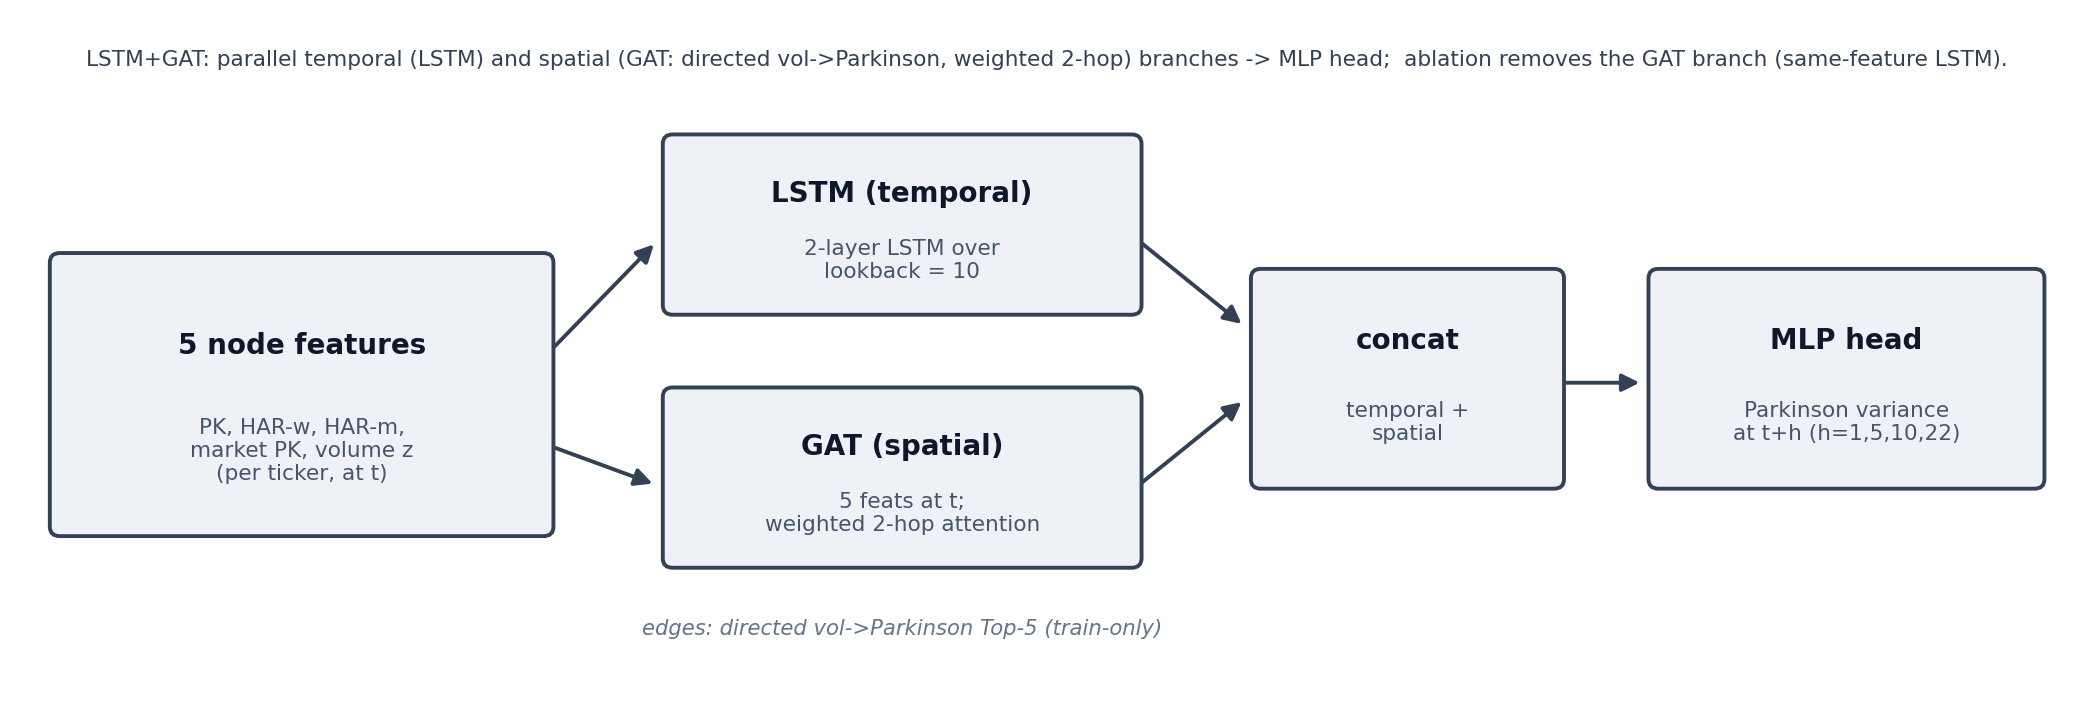
\includegraphics[width=\textwidth]{diagrams/soict_harlstmgat.png}
\caption{LSTM+GAT: a per-node LSTM temporal branch and a GAT spatial branch (directed volume$\to$Parkinson
Top-5 weighted two-hop attention) are concatenated into an MLP head; the leave-one-out comparison removes the
GAT branch to give the same-feature LSTM.}
\label{fig:arch}
\end{figure}

\section{Data}
Two panels are used with the Parkinson target: \textbf{VN30} (primary) and \textbf{VN100} (vnstock). Both use the masked panel of Sec.~3 with the five features, a single chronological
split and per-ticker standardization fit on training rows only.

\section{Experiments}
We compare HAR-X, the five-feature LSTM and the five-feature LSTM+GAT (directed volume$\to$Parkinson weighted
two-hop) on VN30 and VN100 over the masked panel at horizons $\{1,5,10,22\}$, reporting all
five metrics and the two targeted date-clustered DM contrasts (LSTM vs HAR-X, LSTM+GAT vs LSTM).

\section{Results}
Point-error metrics are scaled (MSE $\times10^{-7}$, RMSE $\times10^{-4}$, MAE $\times10^{-4}$); QLIKE and
$R^2$ unscaled. For the learned models each value is the mean of the seed-level metrics over five seeds; the
QLIKE column additionally reports the per-seed standard deviation ($\pm$). HAR-X and GARCH are deterministic.
All values are read from \texttt{results/masked\_rich\_floor1e2/}. Row order is
HAR-X $\to$ GARCH $\to$ LSTM $\to$ LSTM+GAT. Tables~\ref{tab:vn100} and~\ref{tab:vn30} report all five metrics;
Table~\ref{tab:dm} reports the two targeted date-clustered DM contrasts on QLIKE and MAE. The primary horizons
$h1$/$h5$ appear first; the extended horizons $h10$/$h22$ appear in the lower block of each table.

\begin{table}[t]
\centering
\caption{VN100 (46{,}308 masked obs over 454 test dates at $h1$; learned models: seed mean, QLIKE
$\pm$~per-seed std). Lower is better for MSE/RMSE/MAE/QLIKE, higher for $R^2$. $^{\dagger}$~marks metrics where LSTM+GAT improves over the no-graph LSTM. MSE $\times10^{-7}$, RMSE $\times10^{-4}$, MAE $\times10^{-4}$.}
\label{tab:vn100}
\footnotesize
\setlength{\tabcolsep}{5pt}
% AUTHORITATIVE: generated by scripts/paper/build_final_tables.py (do not hand-edit numbers)
\begin{tabular}{llccccc}
\toprule
$h$ & Model & MSE & RMSE & MAE & QLIKE & $R^2$ \\
\midrule
1 & HAR-X & \textbf{2.367} & \textbf{4.865} & 2.898 & \textbf{0.5115} & \textbf{0.2236} \\
1 & GARCH & 3.816 & 6.178 & 4.538 & 0.7577 & -0.2519 \\
1 & LSTM & 2.386 & 4.885 & 2.774 & 0.6229\,$\pm$.074 & 0.2172 \\
1 & LSTM+GAT & 2.371 & 4.869 & \textbf{2.773} & 0.5504\,$\pm$.020 & 0.2224 \\
\midrule
5 & HAR-X & \textbf{2.606} & \textbf{5.104} & 3.160 & \textbf{0.5633} & \textbf{0.1466} \\
5 & GARCH & 3.814 & 6.176 & 4.546 & 0.7420 & -0.2493 \\
5 & LSTM & 2.649 & 5.147 & 3.142 & 0.6021\,$\pm$.039 & 0.1324 \\
5 & LSTM+GAT & 2.634 & 5.132 & \textbf{3.126} & 0.5759\,$\pm$.012 & 0.1373 \\
\midrule
10 & HAR-X & \textbf{2.754} & \textbf{5.248} & 3.306 & \textbf{0.6023} & \textbf{0.0978} \\
10 & GARCH & 3.891 & 6.238 & 4.582 & 0.7605 & -0.2745 \\
10 & LSTM & 2.796 & 5.288 & \textbf{3.297} & 0.6100\,$\pm$.008 & 0.0842 \\
10 & LSTM+GAT & 2.812 & 5.303 & 3.342 & 0.6103\,$\pm$.003 & 0.0789 \\
\midrule
22 & HAR-X & \textbf{2.891} & \textbf{5.377} & \textbf{3.486} & \textbf{0.6405} & \textbf{0.0544} \\
22 & GARCH & 3.854 & 6.208 & 4.568 & 0.7450 & -0.2603 \\
22 & LSTM & 2.988 & 5.466 & 3.507 & 0.6525\,$\pm$.001 & 0.0229 \\
22 & LSTM+GAT & 3.029 & 5.504 & 3.600 & 0.6576\,$\pm$.002 & 0.0093 \\
\bottomrule
\end{tabular}

\end{table}

\begin{table}[t]
\centering
\caption{VN30 (10{,}106 masked obs over 326 test dates at $h1$; learned: seed mean, QLIKE $\pm$~per-seed std). $^{\dagger}$~as in Table~1. Same scaling as
Table~\ref{tab:vn100}.}
\label{tab:vn30}
\footnotesize
\setlength{\tabcolsep}{5pt}
% AUTHORITATIVE: generated by scripts/paper/build_final_tables.py (do not hand-edit numbers)
\input{generated/tab_vn30.tex}
\end{table}

\begin{table}[t]
\centering
\caption{Targeted date-clustered DM contrasts on the 5-seed ensemble forecast ($p$-value; favoured model in parentheses; bold if $p<0.05$; unadjusted).
H=HAR-X, L=LSTM, G=LSTM+GAT, on QLIKE and MAE.}
\label{tab:dm}
\footnotesize
\setlength{\tabcolsep}{5pt}
\begin{tabular}{ll cc cc}
\toprule
& & \multicolumn{2}{c}{LSTM vs HAR-X} & \multicolumn{2}{c}{LSTM+GAT vs LSTM} \\
\cmidrule(lr){3-4}\cmidrule(lr){5-6}
Panel & $h$ & QLIKE & MAE & QLIKE & MAE \\
\midrule
VN100 & 1  & \textbf{.001 (H)} & \textbf{$<$.001 (L)} & \textbf{$<$.001 (G)} & .542 (L) \\
VN100 & 5  & .402 (H) & .077 (L) & \textbf{$<$.001 (G)} & \textbf{$<$.001 (G)} \\
VN100 & 10 & .730 (H) & .523 (L) & .453 (L) & \textbf{$<$.001 (L)} \\
VN100 & 22 & .407 (H) & .618 (H) & .140 (L) & \textbf{$<$.001 (L)} \\
\midrule
VN30 & 1  & \textbf{$<$.001 (H)} & \textbf{.003 (L)} & \textbf{$<$.001 (G)} & \textbf{$<$.001 (L)} \\
VN30 & 5  & .122 (H) & \textbf{$<$.001 (H)} & .280 (L) & \textbf{$<$.001 (G)} \\
VN30 & 10 & .249 (H) & .614 (H) & .162 (G) & .331 (L) \\
VN30 & 22 & .520 (H) & .061 (H) & .625 (G) & \textbf{$<$.001 (L)} \\
\bottomrule
\end{tabular}
\end{table}

\textbf{Short-horizon results ($h1$, $h5$).} HAR-X has the lowest QLIKE in all four short-horizon cells, well
below the seed-mean QLIKE of the learned models. At VN100 $h1$ the LSTM+GAT has the lowest MAE, while HAR-X has the lowest MSE, RMSE and $R^2$; the
LSTM+GAT has a higher QLIKE than HAR-X (seed mean $0.5504$ vs $0.5115$). By DM the deep models have a lower
MAE than HAR-X ($p<0.001$) and the LSTM+GAT a significantly lower QLIKE than the no-graph LSTM ($p<0.001$). At
VN100 $h5$ HAR-X has the lowest QLIKE and the LSTM+GAT the lowest MAE; the LSTM+GAT again has a lower QLIKE than
the LSTM ($p<0.001$). At VN30 $h1$ HAR-X has the lowest QLIKE ($0.5159$, against deep seed means of
$0.66$--$0.70$) and the LSTM the lowest MAE ($p=0.003$ vs HAR-X); the LSTM+GAT has a lower QLIKE than the
no-graph LSTM ($p<0.001$). At VN30 $h5$ HAR-X has the lowest value on all five metrics and the graph's QLIKE
advantage over the LSTM is not significant ($p=0.28$). The per-seed QLIKE standard deviation of the learned
models ($0.02$--$0.07$) is comparable to the graph-vs-LSTM gap, so this is an ensemble-level effect within seed
noise.

\textbf{Extended-horizon results ($h10$, $h22$).} HAR-X has the lowest MSE, RMSE, QLIKE and $R^2$ on both
panels at both horizons; the LSTM has the lowest MAE at VN100 $h10$, and HAR-X the lowest MAE in the other
extended-horizon cells. By DM the LSTM+GAT-vs-LSTM QLIKE difference is not significant at $h10$ or $h22$ on
either panel, and no learned model has a significantly lower QLIKE than HAR-X.

\textbf{GARCH benchmark.} GARCH(1,1) has a higher MSE, RMSE, MAE and QLIKE and a lower $R^2$ than HAR-X at
every horizon on both panels, with a negative $R^2$ on both; its QLIKE is higher than HAR-X's under the
date-clustered DM test in all eight cells ($p<0.001$, except VN30 $h22$ where $p=0.001$). GARCH is a frozen-train forecast: a single conditional-variance path is projected from the end of training (persistence capped at 0.999 by variance targeting), so it cannot adapt to the level shifts that HAR-X re-estimates each day, and its error is correspondingly higher.

\textbf{Per-metric ranking.} No single metric determines the ordering, so all five are reported with equal
weight: HAR-X has the lowest QLIKE at every horizon on both panels, with no learned model significantly lower
at any horizon; the deep and graph models have the lowest point error (MAE) at some short horizons on VN100;
and HAR-X has the lowest MSE and RMSE at every horizon.

\section{Out-of-sample extension: broader Vietnamese universe (HOSE, HNX)}\label{sec:oos}
HOSE and HNX daily OHLCV were crawled and processed to the same Parkinson-variance target as VN30/VN100. A
liquidity-and-history screen (at least 250 rows per ticker and at most 50\% zero-variance days) was applied,
leaving the modelled universe reported by the \texttt{num\_nodes} field of each results file: 352 tickers on
HOSE and 154 on HNX (153 at $h22$). This universe was not used to design the model or to select any
configuration, so it is an untouched out-of-sample check. The same main configuration and protocol as
VN30/VN100 are used: the same five node features, the masked panel, the z-score$+$linear output with a
relative floor at $10^{-2}$ times the per-node training mean, five seeds and the date-clustered DM test. The
absolute QLIKE is higher than on VN30/VN100 because these panels are far less liquid; many low-range days
remain even after screening, which inflates the QLIKE level for every model.

\begin{table}[t]
\centering
\caption{HOSE (186{,}944 masked obs over 572 test dates at $h1$; learned models: seed mean, QLIKE
$\pm$~per-seed std). Lower is better for MSE/RMSE/MAE/QLIKE, higher for $R^2$. $^{\dagger}$~marks metrics where LSTM+GAT improves over the no-graph
LSTM. MSE $\times10^{-7}$, RMSE $\times10^{-4}$, MAE $\times10^{-4}$.}
\label{tab:hose}
\footnotesize
\setlength{\tabcolsep}{5pt}
% AUTHORITATIVE: generated by scripts/paper/build_final_tables.py (do not hand-edit numbers)
\begin{tabular}{llccccc}
\toprule
$h$ & Model & MSE & RMSE & MAE & QLIKE & $R^2$ \\
\midrule
1 & HAR-X & 3.299 & 5.744 & 3.309 & \textbf{1.2342} & 0.1854 \\
1 & GARCH & 18.495 & 13.600 & 5.878 & 1.4865 & -3.5660 \\
1 & LSTM & \textbf{3.275} & \textbf{5.722} & \textbf{3.224} & 1.3350\,$\pm$.146 & \textbf{0.1916} \\
1 & LSTM+GAT & 3.278 & 5.726 & 3.237 & 1.3031\,$\pm$.097 & 0.1907 \\
\midrule
5 & HAR-X & \textbf{3.610} & \textbf{6.009} & 3.647 & \textbf{1.2963} & \textbf{0.1091} \\
5 & GARCH & 6.151 & 7.843 & 5.223 & 1.4767 & -0.5179 \\
5 & LSTM & 3.633 & 6.028 & \textbf{3.579} & 1.3652\,$\pm$.046 & 0.1034 \\
5 & LSTM+GAT & 3.654 & 6.045 & 3.685 & 1.3202\,$\pm$.022 & 0.0982 \\
\midrule
10 & HAR-X & \textbf{3.744} & \textbf{6.118} & \textbf{3.807} & \textbf{1.3387} & \textbf{0.0774} \\
10 & GARCH & 5.503 & 7.418 & 5.125 & 1.4871 & -0.3563 \\
10 & LSTM & 3.830 & 6.188 & 3.900 & 1.3530\,$\pm$.012 & 0.0562 \\
10 & LSTM+GAT & 3.805 & 6.169 & 3.873 & 1.3388\,$\pm$.002 & 0.0621 \\
\midrule
22 & HAR-X & \textbf{3.878} & \textbf{6.227} & \textbf{3.995} & \textbf{1.3820} & \textbf{0.0449} \\
22 & GARCH & 5.592 & 7.478 & 5.141 & 1.4880 & -0.3773 \\
22 & LSTM & 3.989 & 6.316 & 4.071 & 1.3854\,$\pm$.010 & 0.0175 \\
22 & LSTM+GAT & 4.004 & 6.328 & 4.121 & 1.3842\,$\pm$.004 & 0.0137 \\
\bottomrule
\end{tabular}

\end{table}

\begin{table}[t]
\centering
\caption{HNX (62{,}004 masked obs over 489 test dates at $h1$; learned models: seed mean, QLIKE
$\pm$~per-seed std). $^{\dagger}$~as in Table~\ref{tab:hose}. Same scaling as Table~\ref{tab:hose}.}
\label{tab:hnx}
\footnotesize
\setlength{\tabcolsep}{5pt}
% AUTHORITATIVE: generated by scripts/paper/build_final_tables.py (do not hand-edit numbers)
\begin{tabular}{llccccc}
\toprule
$h$ & Model & MSE & RMSE & MAE & QLIKE & $R^2$ \\
\midrule
1 & HAR-X & 13.986 & 11.826 & 6.549 & 1.8717 & 0.2154 \\
1 & GARCH & 21.336 & 14.607 & 9.503 & 2.1065 & -0.1969 \\
1 & LSTM & \textbf{13.736} & \textbf{11.720} & 6.443 & 1.8205\,$\pm$.014 & \textbf{0.2294} \\
1 & LSTM+GAT & 13.738 & 11.721 & \textbf{6.422} & \textbf{1.8152\,$\pm$.004} & 0.2293 \\
\midrule
5 & HAR-X & 15.495 & 12.448 & 7.123 & 1.9402 & 0.1273 \\
5 & GARCH & 19.960 & 14.128 & 9.268 & 2.1052 & -0.1241 \\
5 & LSTM & \textbf{15.441} & \textbf{12.426} & \textbf{7.107} & \textbf{1.9331\,$\pm$.002} & \textbf{0.1304} \\
5 & LSTM+GAT & 15.494 & 12.448 & 7.198 & 1.9370\,$\pm$.004 & 0.1274 \\
\midrule
10 & HAR-X & \textbf{15.977} & \textbf{12.640} & \textbf{7.361} & 1.9904 & \textbf{0.0970} \\
10 & GARCH & 19.832 & 14.083 & 9.301 & 2.2020 & -0.1209 \\
10 & LSTM & 16.023 & 12.658 & 7.486 & 1.9848\,$\pm$.004 & 0.0944 \\
10 & LSTM+GAT & 15.999 & 12.649 & 7.455 & \textbf{1.9832\,$\pm$.004} & 0.0958 \\
\midrule
22 & HAR-X & \textbf{16.554} & \textbf{12.866} & \textbf{7.635} & 2.0391 & \textbf{0.0681} \\
22 & GARCH & 18.948 & 13.765 & 9.107 & 2.1254 & -0.0667 \\
22 & LSTM & 16.679 & 12.915 & 7.872 & 2.0322\,$\pm$.003 & 0.0611 \\
22 & LSTM+GAT & 16.601 & 12.884 & 7.769 & \textbf{2.0287\,$\pm$.001} & 0.0655 \\
\bottomrule
\end{tabular}

\end{table}

\begin{table}[t]
\centering
\caption{Out-of-sample date-clustered DM contrasts on HOSE and HNX ($p$-value; favoured model in
parentheses; bold if $p<0.05$). H=HAR-X, L=LSTM, G=LSTM+GAT, on QLIKE and MAE.}
\label{tab:dmext}
\footnotesize
\setlength{\tabcolsep}{4pt}
\begin{tabular}{ll cc cc cc}
\toprule
& & \multicolumn{2}{c}{LSTM vs HAR-X} & \multicolumn{2}{c}{LSTM+GAT vs HAR-X} & \multicolumn{2}{c}{LSTM+GAT vs LSTM} \\
\cmidrule(lr){3-4}\cmidrule(lr){5-6}\cmidrule(lr){7-8}
Panel & $h$ & QLIKE & MAE & QLIKE & MAE & QLIKE & MAE \\
\midrule
HOSE & 1  & .553 (H) & \textbf{$<$.001 (L)} & .593 (H) & \textbf{$<$.001 (G)} & .649 (G) & \textbf{$<$.001 (L)} \\
HOSE & 5  & .163 (H) & \textbf{$<$.001 (L)} & .384 (H) & \textbf{.005 (H)} & .095 (G) & \textbf{$<$.001 (L)} \\
HOSE & 10 & .674 (L) & \textbf{$<$.001 (H)} & .343 (G) & \textbf{$<$.001 (H)} & .108 (G) & \textbf{$<$.001 (G)} \\
HOSE & 22 & .442 (L) & \textbf{.020 (H)} & .712 (G) & \textbf{$<$.001 (H)} & .080 (L) & \textbf{$<$.001 (L)} \\
\midrule
HNX & 1  & \textbf{$<$.001 (L)} & \textbf{$<$.001 (L)} & \textbf{$<$.001 (G)} & \textbf{$<$.001 (G)} & .560 (L) & \textbf{$<$.001 (G)} \\
HNX & 5  & \textbf{.050 (L)} & .404 (L) & .178 (G) & \textbf{$<$.001 (H)} & \textbf{.023 (L)} & \textbf{$<$.001 (L)} \\
HNX & 10 & .065 (L) & \textbf{$<$.001 (H)} & \textbf{.022 (G)} & \textbf{$<$.001 (H)} & \textbf{.015 (G)} & \textbf{$<$.001 (G)} \\
HNX & 22 & .094 (L) & \textbf{$<$.001 (H)} & \textbf{.016 (G)} & \textbf{$<$.001 (H)} & \textbf{.031 (G)} & \textbf{$<$.001 (G)} \\
\bottomrule
\end{tabular}
\end{table}

\textbf{Interpretation.} On HNX the deep models attain a significantly lower QLIKE than HAR-X at $h1$
(LSTM and LSTM+GAT, $p<0.001$), $h10$ (LSTM+GAT, $p=0.022$) and $h22$ (LSTM+GAT, $p=0.016$), with the LSTM
borderline at $h5$ ($p=0.050$); the LSTM+GAT also has a significantly lower QLIKE than the no-graph LSTM at
$h10$ ($p=0.015$) and $h22$ ($p=0.031$). The temporal and graph value that is absent on the liquid VN30/VN100
blue chips thus appears on the broader, less-liquid HNX universe. On HOSE no learned model differs
significantly from HAR-X on QLIKE at any horizon ($p\ge0.16$); the deep models still have the lowest MAE at
$h1$ ($p<0.001$), which reverses at $h10$/$h22$ where HAR-X has the lower MAE ($p<0.001$--$0.020$). GARCH is
far worse on both exchanges, with a negative $R^2$ (down to $-3.6$ on HOSE $h1$) and a significantly
higher QLIKE than HAR-X in every cell ($p<0.001$), consistent with a single frozen-train conditional-variance
path that cannot track the panels' level shifts.
These are out-of-sample observations from a single configuration on one holdout; they motivate, but do not by
themselves establish, the deep and graph advantage on less-liquid Vietnamese equities.

\section{Cross-market out-of-sample check: S\&P 500}\label{sec:sp500}
As a developed-market contrast to the Vietnamese panels, we apply the same configuration and protocol,
without any retuning, to the S\&P 500. Daily OHLCV for the constituents were obtained from a public source and
processed to the same Parkinson-variance target; the same liquidity-and-history screen (at least 250 rows per
ticker and at most 50\% zero-variance days) leaves 440 tickers at $h1$ (714{,}520 masked obs over 1{,}624 test
dates, decreasing to 438 tickers at $h22$). This large, highly liquid universe was not used to design the model
or to select any configuration, so it is a second untouched out-of-sample check on a different market.

\begin{table}[t]
\centering
\caption{S\&P 500 (714{,}520 masked obs over 1{,}624 test dates at $h1$; learned models: seed mean, QLIKE
$\pm$~per-seed std). Lower is better for MSE/RMSE/MAE/QLIKE, higher for $R^2$. $^{\dagger}$~marks metrics where LSTM+GAT improves over the no-graph
LSTM. MSE $\times10^{-7}$, RMSE $\times10^{-4}$, MAE $\times10^{-4}$.}
\label{tab:sp500}
\footnotesize
\setlength{\tabcolsep}{5pt}
% AUTHORITATIVE: generated by scripts/paper/build_final_tables.py (do not hand-edit numbers)
\begin{tabular}{llccccc}
\toprule
$h$ & Model & MSE & RMSE & MAE & QLIKE & $R^2$ \\
\midrule
1 & HAR-X & \textbf{6.189} & \textbf{7.867} & 2.364 & \textbf{0.3590} & \textbf{0.3198} \\
1 & GARCH & 13.619 & 11.670 & 5.491 & 0.8329 & -0.4970 \\
1 & LSTM & 6.357 & 7.973 & 2.392 & 0.4619\,$\pm$.103 & 0.3012 \\
1 & LSTM+GAT & 6.332 & 7.957 & \textbf{2.336} & 0.4152\,$\pm$.040 & 0.3040 \\
\midrule
5 & HAR-X & 8.087 & 8.993 & 2.695 & \textbf{0.4171} & 0.1110 \\
5 & GARCH & 14.043 & 11.850 & 5.578 & 0.8327 & -0.5436 \\
5 & LSTM & 7.951 & 8.917 & 2.667 & 0.5917\,$\pm$.213 & 0.1260 \\
5 & LSTM+GAT & \textbf{7.929} & \textbf{8.904} & \textbf{2.573} & 0.5257\,$\pm$.030 & \textbf{0.1285} \\
\midrule
10 & HAR-X & 8.977 & 9.475 & 2.847 & \textbf{0.4642} & 0.0152 \\
10 & GARCH & 13.580 & 11.653 & 5.476 & 0.8415 & -0.4898 \\
10 & LSTM & 8.631 & 9.290 & 2.894 & 0.5092\,$\pm$.012 & 0.0531 \\
10 & LSTM+GAT & \textbf{8.534} & \textbf{9.238} & \textbf{2.761} & 0.5299\,$\pm$.032 & \textbf{0.0638} \\
\midrule
22 & HAR-X & 9.655 & 9.826 & 2.988 & \textbf{0.5848} & -0.0578 \\
22 & GARCH & 13.119 & 11.454 & 5.384 & 0.8241 & -0.4373 \\
22 & LSTM & 9.339 & 9.664 & 3.066 & 0.7602\,$\pm$.110 & -0.0232 \\
22 & LSTM+GAT & \textbf{9.305} & \textbf{9.646} & \textbf{2.980} & 0.7755\,$\pm$.102 & \textbf{-0.0195} \\
\bottomrule
\end{tabular}

\end{table}

\begin{table}[t]
\centering
\caption{S\&P 500 date-clustered DM contrasts ($p$-value; favoured model in parentheses; bold if $p<0.05$).
H=HAR-X, L=LSTM, G=LSTM+GAT, on QLIKE and MAE.}
\label{tab:dmsp500}
\footnotesize
\setlength{\tabcolsep}{4pt}
\begin{tabular}{ll cc cc cc}
\toprule
& & \multicolumn{2}{c}{LSTM vs HAR-X} & \multicolumn{2}{c}{LSTM+GAT vs HAR-X} & \multicolumn{2}{c}{LSTM+GAT vs LSTM} \\
\cmidrule(lr){3-4}\cmidrule(lr){5-6}\cmidrule(lr){7-8}
Panel & $h$ & QLIKE & MAE & QLIKE & MAE & QLIKE & MAE \\
\midrule
SP500 & 1  & \textbf{$<$.001 (H)} & .452 (H) & .083 (H) & \textbf{.003 (G)} & \textbf{$<$.001 (G)} & \textbf{$<$.001 (G)} \\
SP500 & 5  & \textbf{$<$.001 (H)} & .264 (L) & \textbf{$<$.001 (H)} & \textbf{.003 (G)} & \textbf{$<$.001 (L)} & \textbf{$<$.001 (G)} \\
SP500 & 10 & \textbf{.035 (H)} & .634 (H) & \textbf{.002 (H)} & .224 (G) & .821 (L) & \textbf{$<$.001 (G)} \\
SP500 & 22 & .179 (H) & .467 (H) & .192 (H) & .865 (G) & .265 (L) & \textbf{$<$.001 (G)} \\
\bottomrule
\end{tabular}
\end{table}

\textbf{Interpretation.} On the S\&P 500 HAR-X has the lowest QLIKE at every horizon, and here the QLIKE gap is
statistically significant: the LSTM has a higher QLIKE than HAR-X at $h1$, $h5$ and $h10$ ($p<0.001$,
$p<0.001$, $p=0.035$) and the LSTM+GAT at $h5$ and $h10$ ($p<0.001$, $p=0.002$), with neither significant at
$h22$. The deep and graph models instead have the advantage on point error: the LSTM+GAT has the lowest MSE,
RMSE and MAE from $h5$ onward and a lower MAE than HAR-X at $h1$ and $h5$ ($p=0.003$), and a lower MAE than the
no-graph LSTM at every horizon ($p<0.001$). The graph lowers QLIKE relative to the no-graph LSTM only at $h1$
($p<0.001$); at $h5$--$h22$ the LSTM+GAT-vs-LSTM QLIKE difference is not in the graph's favour. GARCH is again
far worse, with QLIKE around $0.83$ and a negative $R^2$ (around $-0.5$) at every horizon. The negative $R^2$ at $h22$ for
all models reflects long-horizon regression toward the mean. The pattern across markets is consistent: the deep
and graph models reduce squared and absolute error but do not lower QLIKE below HAR-X on the liquid VN30/VN100,
HOSE and S\&P 500 panels, whereas the learned models' QLIKE advantage appears on the less-liquid HNX universe.

\section{Sensitivity to the volatility proxy}\label{sec:proxy}
The forecast target so far is the Parkinson variance. Parkinson uses only the intraday high--low range and is
valid under zero drift and no opening jumps, so a natural question is whether the model comparison depends on
this choice. We re-run the full pipeline (HAR-X, LSTM, LSTM+GAT; five seeds; the same masked panel, universe and
protocol) with the target replaced by an \emph{indicator-form Yang--Zhang-inspired} per-day variance proxy,
$\sigma^2_{\mathrm{YZ\text{-}ind},t}=r_{o,t}^2+k\,r_{c,t}^2+(1-k)\,\mathrm{RS}_t$ with the overnight return
$r_o=\ln(O_t/C_{t-1})$, the open-to-close return $r_c=\ln(C_t/O_t)$, the Rogers--Satchell term $\mathrm{RS}_t$,
and $k=0.34/(1.34+(n{+}1)/(n{-}1))\approx0.14$ ($n{=}20$). This is a single-day composite in the spirit of the
TradingView ``YZV'' indicator; it is \emph{not} the standard windowed Yang--Zhang~(2000) estimator (which
combines these three variances over a rolling window), so the claim below is a per-day-proxy robustness check,
not a standard-Yang--Zhang result. QLIKE is scale-invariant, so it is comparable across the two targets.

\begin{table}[t]
\centering
\caption{Volatility-proxy robustness: five-seed-mean QLIKE (lower is better) of each model when the target is
the Parkinson variance vs.\ an indicator-form Yang--Zhang-inspired per-day proxy (\emph{not} standard windowed YZ), on the same universe/protocol. Bold marks the
lowest QLIKE per row-block. The lowest-QLIKE model is unchanged under both proxies on the Vietnamese panels (HAR-X on VN30/VN100/HOSE; LSTM+GAT on HNX);
on the S\&P 500 the models tie under the YZ-inspired proxy.}
\label{tab:proxy}
\footnotesize
\setlength{\tabcolsep}{6pt}
\begin{tabular}{llccc}
\toprule
Panel & Target & HAR-X & LSTM & LSTM+GAT \\
\midrule
VN100 & Parkinson & \textbf{0.512} & 0.621 & 0.552 \\
VN100 & YZ-ind. & \textbf{0.527} & 0.640 & 0.540 \\
\midrule
VN30 & Parkinson & \textbf{0.516} & 0.679 & 0.619 \\
VN30 & YZ-ind. & \textbf{0.722} & 0.775 & 0.777 \\
\midrule
HOSE & Parkinson & \textbf{1.244} & 1.310 & 1.355 \\
HOSE & YZ-ind. & \textbf{1.194} & 1.527 & 1.375 \\
\midrule
HNX & Parkinson & 1.872 & 1.821 & \textbf{1.816} \\
HNX & YZ-ind. & 1.635 & 1.650 & \textbf{1.623} \\
\midrule
SP500 & Parkinson & \textbf{0.362} & 0.638 & 0.543 \\
SP500 & YZ-ind. & 0.565 & \textbf{0.553} & 0.562 \\
\bottomrule
\end{tabular}
\end{table}

The lowest-QLIKE model is \emph{identical} under both targets on the four Vietnamese panels: HAR-X on the
liquid VN30, VN100 and HOSE, and the LSTM+GAT on the illiquid HNX. On the S\&P 500 (five seeds) HAR-X is
clearly lowest under Parkinson, while under the YZ-inspired proxy the three models fall within $0.013$ --- inside the
per-seed dispersion --- so they are statistically indistinguishable rather than re-ranked. The same pattern holds at h5/h10/h22 (full results in the accompanying review sheet): HAR-X remains lowest on the liquid panels and a deep model on HNX under both proxies at every horizon. The headline finding --- the linear HAR-X is best on the
liquid large-caps while the graph model attains the lowest QLIKE on the illiquid HNX --- is therefore robust to
the volatility proxy. The YZ-inspired proxy lowers the absolute QLIKE on the less-liquid HOSE and HNX (its
overnight component records variance on the many near-zero-range days that Parkinson floors) but raises the MSE
by roughly three to four times (its overnight jumps are large and not persistent), so it is not a free
improvement. The small LSTM+GAT-vs-LSTM QLIKE contrast is itself proxy-dependent --- significant at VN30 under
Parkinson but not under the YZ-inspired proxy, and reversing sign at HOSE --- consistent with that contrast lying within
the per-seed dispersion reported above. We keep Parkinson as the primary target for its simplicity and split
invariance. A fully clean YZ-inspired-proxy comparison requires split/dividend-adjusted prices: the S\&P 500 series
used here are already adjusted (verified against Yahoo's adjusted close --- the ratio is $1.0000$ with zero
variance across tickers), so its overnight term is uncorrupted, whereas the Vietnamese OHLCV is not adjusted
and its overnight return is winsorized at $\pm0.20$; a fully adjusted Vietnamese comparison is left to future
work.

\section{Discussion}\label{sec:disc}
No learned model has a significantly lower QLIKE than HAR-X at any horizon under the date-clustered DM test,
and HAR-X has the lowest QLIKE seed-mean in every cell on both panels. At $h1$ the deep models have the lowest
MAE on VN100 (LSTM vs HAR-X, $p<0.001$), and the LSTM+GAT has a significantly lower QLIKE than the same-feature
no-graph LSTM at VN30 $h1$, VN100 $h1$ and VN100 $h5$; this graph effect is absent at VN30 $h5$ and at the
longer horizons. Because the per-seed QLIKE standard deviation of the learned models ($0.02$--$0.07$) is of the
same order as these graph-vs-LSTM differences, and the DM test is computed on the five-seed ensemble forecast,
the graph effect is best read as an ensemble-level regularity rather than a robust per-seed improvement. At
$h10$ and $h22$ HAR-X has the lowest MSE, RMSE, QLIKE and $R^2$. The ranking is metric- and horizon-dependent,
which is why all five metrics are reported with equal weight. The date-clustered DM test matters for these
conclusions: a naive per-observation test on this cross-sectionally dependent panel inflates the statistic by
roughly the square root of the number of stocks, so a difference that is not significant per date can appear
significant per observation. \textbf{Multiplicity.} We report per-metric DM contrasts without a
multiple-comparison correction; the headline conclusion is a set of \emph{null} results (no learned model
significantly beats HAR-X on QLIKE), which a correction would only reinforce, while the significant
graph-vs-LSTM contrasts should be read as unadjusted exploratory findings. \textbf{Capacity.} The LSTM+GAT
adds a graph branch and its parameters to the no-graph LSTM, so the leave-one-out contrast measures the effect
of adding the implemented graph branch, not of graph structure at matched capacity.

\section{Conclusion}
For daily Parkinson-variance forecasting on the Vietnamese market, evaluated with the same features, the same
masked panel and the same date-clustered Diebold--Mariano inference, no learned model has a significantly lower
QLIKE than HAR-X at any horizon, and HAR-X has the lowest QLIKE seed-mean in every cell on both panels. At the
short horizons ($h1$, $h5$) the deep models have the lowest MAE on VN100, and the directed volume$\to$Parkinson
weighted graph gives the LSTM+GAT a significantly lower QLIKE than the same-feature no-graph LSTM at VN30 $h1$,
VN100 $h1$ and VN100 $h5$ --- an ensemble-level difference of the same order as the learned models' per-seed
QLIKE dispersion, and absent at VN30 $h5$; at the extended horizons ($h10$, $h22$) HAR-X has the lowest MSE,
RMSE, QLIKE and $R^2$, and the graph's QLIKE difference from the no-graph LSTM is not significant. The ranking
is metric- and horizon-dependent, so all five metrics are reported with equal weight.

Across four
Vietnamese panels and the S\&P 500, the learned models reduce squared and absolute error on the liquid
large-cap universes but lower QLIKE below HAR-X only on the less-liquid HNX exchange, so any deep or graph
advantage on QLIKE is market- and liquidity-dependent rather than universal.

\begin{thebibliography}{99}
\bibitem{corsi2009} Corsi, F.: A simple approximate long-memory model of realized volatility. J. Financial Econometrics \textbf{7}(2), 174--196 (2009)
\bibitem{parkinson1980} Parkinson, M.: The extreme value method for estimating the variance of the rate of return. J. Business \textbf{53}(1), 61--65 (1980)
\bibitem{lstm1997} Hochreiter, S., Schmidhuber, J.: Long short-term memory. Neural Computation \textbf{9}(8), 1735--1780 (1997)
\bibitem{gat2018} Veli\v{c}kovi\'c, P., et al.: Graph attention networks. In: ICLR (2018)
\bibitem{dm1995} Diebold, F.X., Mariano, R.S.: Comparing predictive accuracy. J. Business \& Economic Statistics \textbf{13}(3), 253--263 (1995)
\bibitem{hln1997} Harvey, D., Leybourne, S., Newbold, P.: Testing the equality of prediction mean squared errors. Int. J. Forecasting \textbf{13}(2), 281--291 (1997)
\bibitem{patton2011} Patton, A.J.: Volatility forecast comparison using imperfect volatility proxies. J. Econometrics \textbf{160}(1), 246--256 (2011)
\bibitem{harq2016} Bollerslev, T., Patton, A.J., Quaedvlieg, R.: Exploiting the errors: a simple approach for improved volatility forecasting. J. Econometrics \textbf{192}(1), 1--18 (2016)
\bibitem{chen2022} Chen, Q., Robert, C.-Y.: Multivariate realized volatility forecasting with graph neural network. In: ACM ICAIF (2022). arXiv:2112.09015
\bibitem{gnnhar2025} Zhang, C., Pu, X., Cucuringu, M., Dong, X.: Forecasting realized volatility with spillover effects: perspectives from graph neural networks (2025). arXiv:2308.01419
\bibitem{dy2012} Diebold, F.X., Yilmaz, K.: Better to give than to receive: predictive directional measurement of volatility spillovers. Int. J. Forecasting \textbf{28}(1), 57--66 (2012)
\bibitem{audrino2025} Audrino, F., Chassot, J.: HARd to beat: the overlooked impact of rolling windows in the era of machine learning. Int. J. Forecasting (2025). arXiv:2406.08041
\end{thebibliography}

\end{document}
